\mode*

\mode<all>{\mode*

\section[Hash functions]{What was a hash function now again?}

%\begin{frame}
%  \begin{definition}[One-way function\footfullcite{GoldreichFOC-1}]
%    \begin{itemize}
%      \item Let \(h\colon \{0,1\}^*\to \{0,1\}^*\).
%      \item \(h\) is \emph{one-way} if
%        \begin{enumerate}
%          \item there exists an efficient algorithm \(A\) such that \(A(x) 
%              = h(x)\);
%          \item for every efficient algorithm \(A^\prime\), every positive 
%            polynomial \(p(\cdot)\) and all sufficiently large \(n\)'s
%            \[\Prob{A^\prime(h(x), 1^n) \in h^{-1}(h(x))} < \frac{1}{p(n)}\]
%        \end{enumerate}
%    \end{itemize}
%  \end{definition}
%\end{frame}

\begin{frame}
  \begin{definition}[Preimage resistance {[one way]}]
    \begin{description}
      \item[Input] hash function~\(H\), value~\(y\).
      \item[Output] Any \(x\) such that \(H(x) = y\).
    \end{description}
  \end{definition}

  \begin{definition}[Second preimage resistance {[weak collision resistance]}]
    \begin{description}
      \item[Input] hash function~\(H\), value \(x\).
      \item[Output] Any value \(x'\) such that \(H(x) = H(x')\).
    \end{description}
  \end{definition}

  \begin{definition}[Collision resistance {[strong collision resistance]}]
    \begin{description}
      \item[Input] hash function~\(H\).
      \item[Output] Any two \(x, x'\) such that \(H(x) = H(x')\).
    \end{description}
  \end{definition}
\end{frame}

}


\section{Fingerprinting}

\begin{frame}
  \begin{definition}[Compressing]
    \begin{itemize}
      \item Function~\(f\colon \{0, 1\}^{l}\to \{0, 1\}^{l'}\)
      \item We can have \(l > l'\).
    \end{itemize}
  \end{definition}

  \pause

  \begin{remark}
    \begin{itemize}
      \item Most hash functions are compressing.
    \end{itemize}
  \end{remark}
\end{frame}

\begin{frame}[fragile]
  \begin{example}[Compressing]
    \begin{itemize}
      \begin{minted}{text}
(1|11:27)dbosk@X1:WinDev2007Eval
$ du WinDev2007Eval-disk001.vdi
43G     WinDev2007Eval-disk001.vdi
(0|11:28)dbosk@X1:WinDev2007Eval
$ sha256sum WinDev2007Eval-disk001.vdi
5260fe9713a5b6341aca8d7e61c9cdb9bb50ee9f5f0bc15e5427a07397df9d95  WinDev2007Eval-disk001.vdi
(0|11:32)dbosk@X1:WinDev2007Eval
$
      \end{minted}
    \end{itemize}
  \end{example}
\end{frame}

\begin{frame}
  \begin{block}{Requirements}
    \begin{description}
      \item[Compressing property] to make the fingerprint small.
      \item[Collision resistance] to reduce likelihood of collisions.
    \end{description}
  \end{block}
\end{frame}

\subsection{BitTorrent}

\begin{frame}
  \begin{figure}
    \begin{subfigure}{0.45\columnwidth}
      \centering
      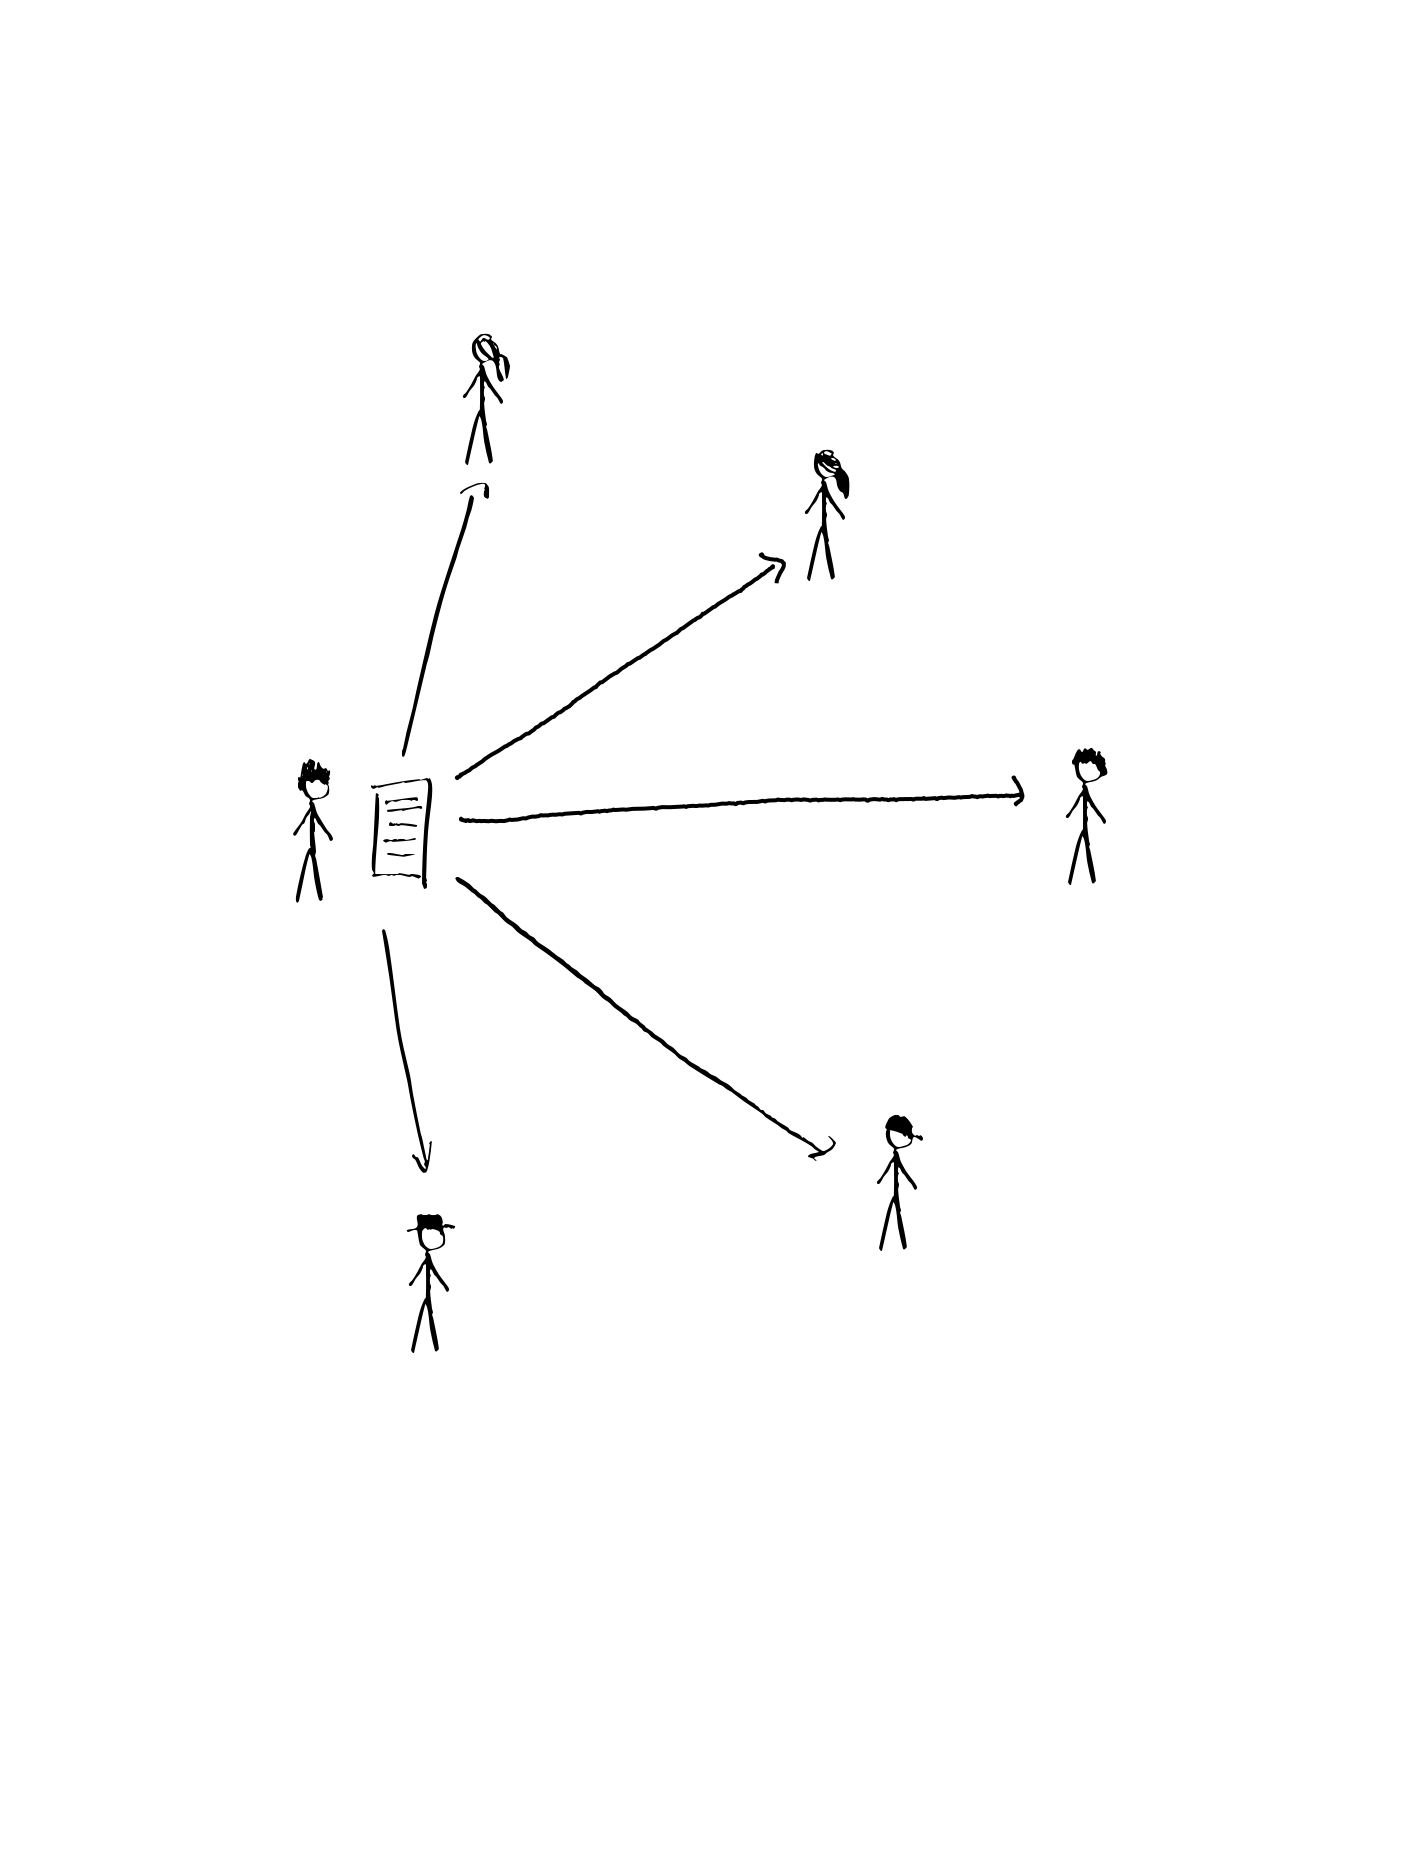
\includegraphics[width=\columnwidth]{fig/centralized.pdf}
      \caption{Centralized}
    \end{subfigure}
    \hfill
    \begin{subfigure}{0.45\columnwidth}
      \centering
      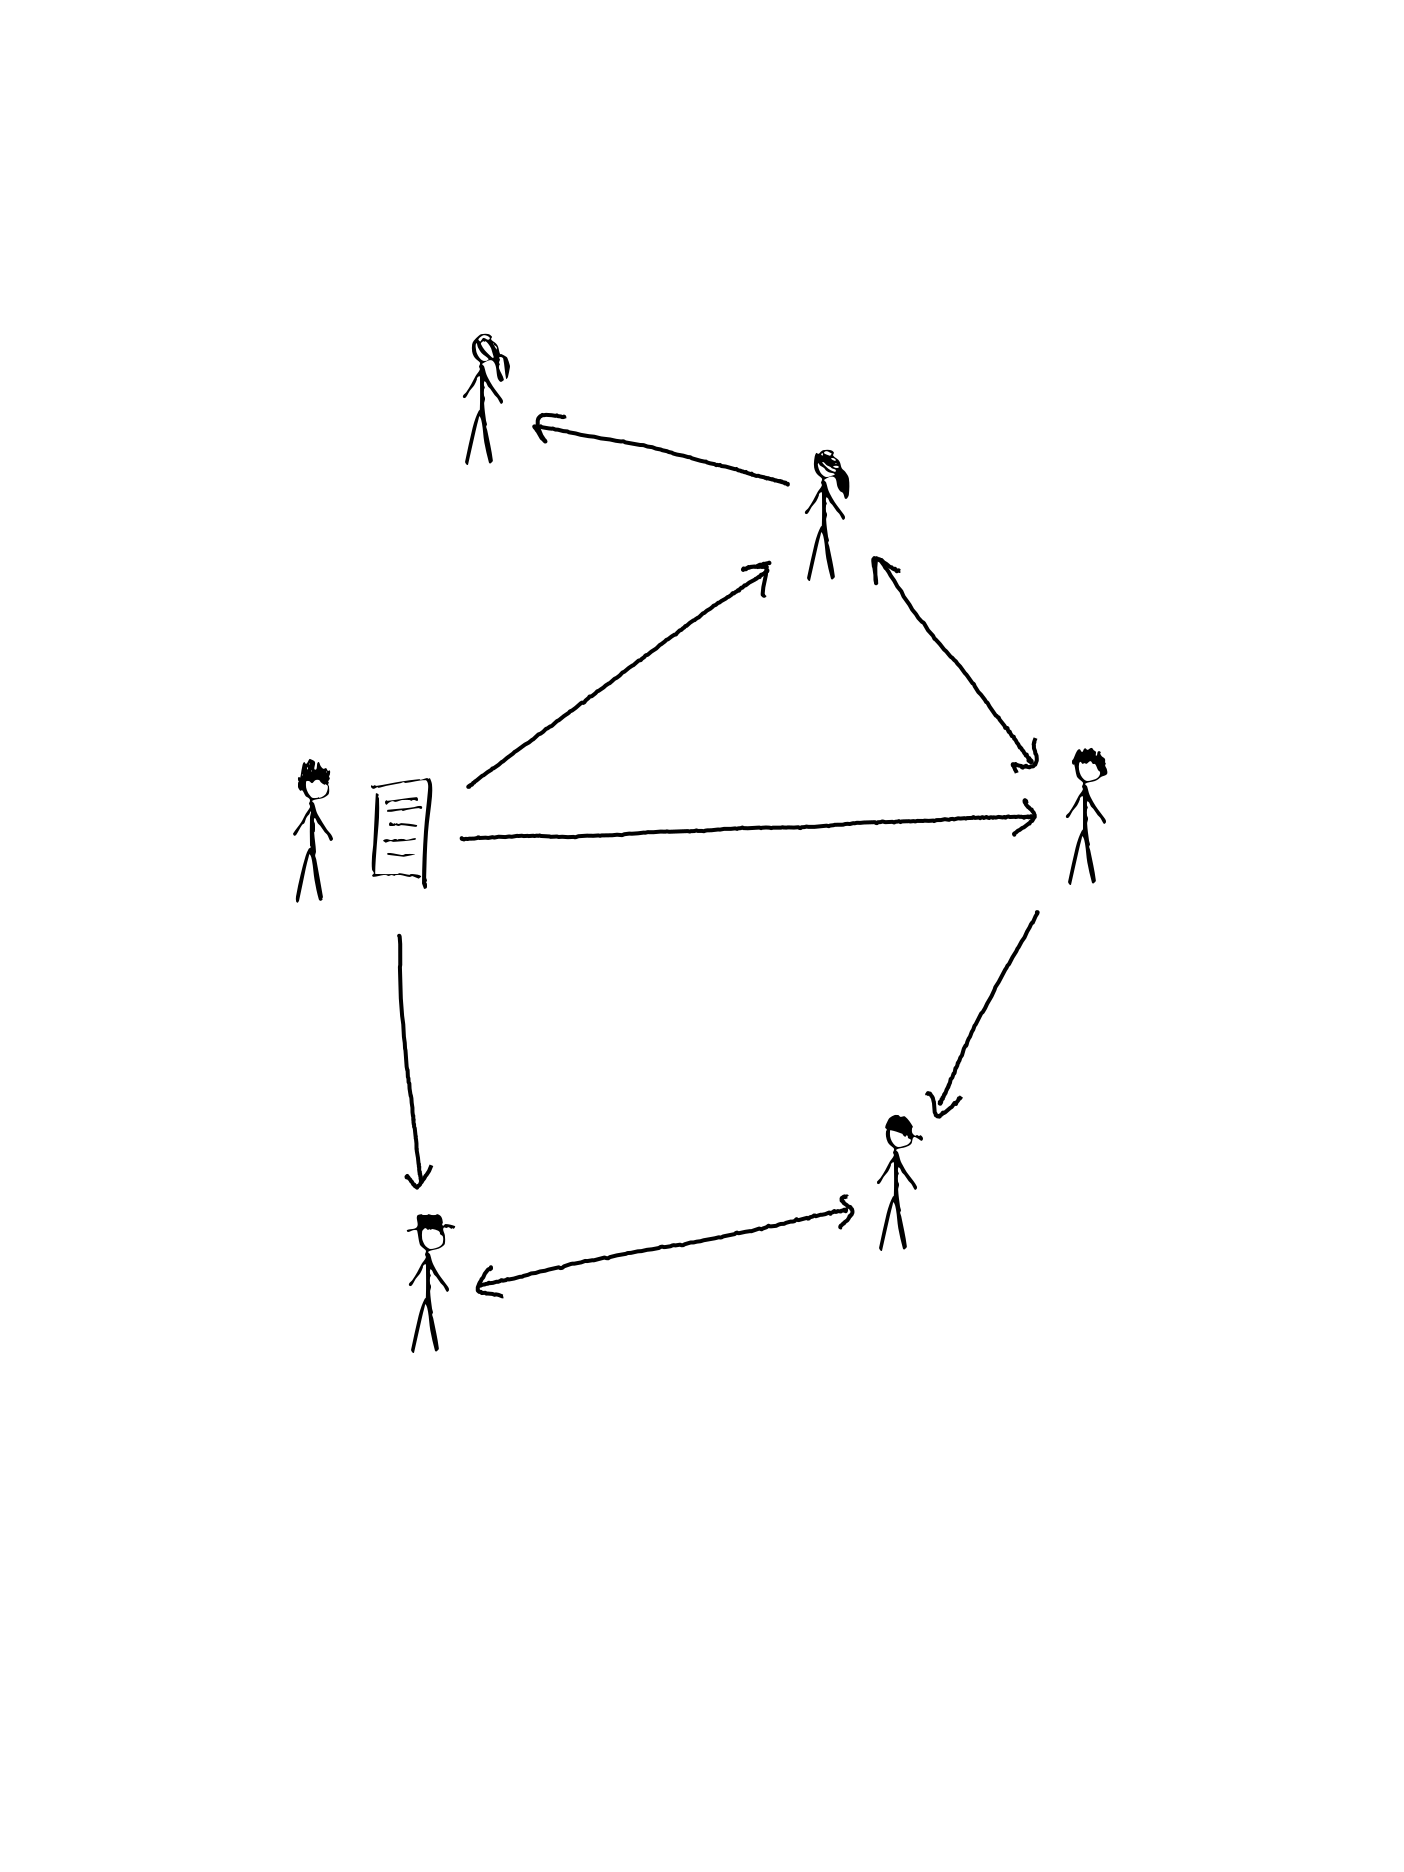
\includegraphics[width=\columnwidth]{fig/p2p.pdf}
      \caption{Peer-to-peer (P2P)}
    \end{subfigure}
  \end{figure}
\end{frame}

\begin{frame}
  \begin{figure}
    \begin{subfigure}{0.45\columnwidth}
      \centering
      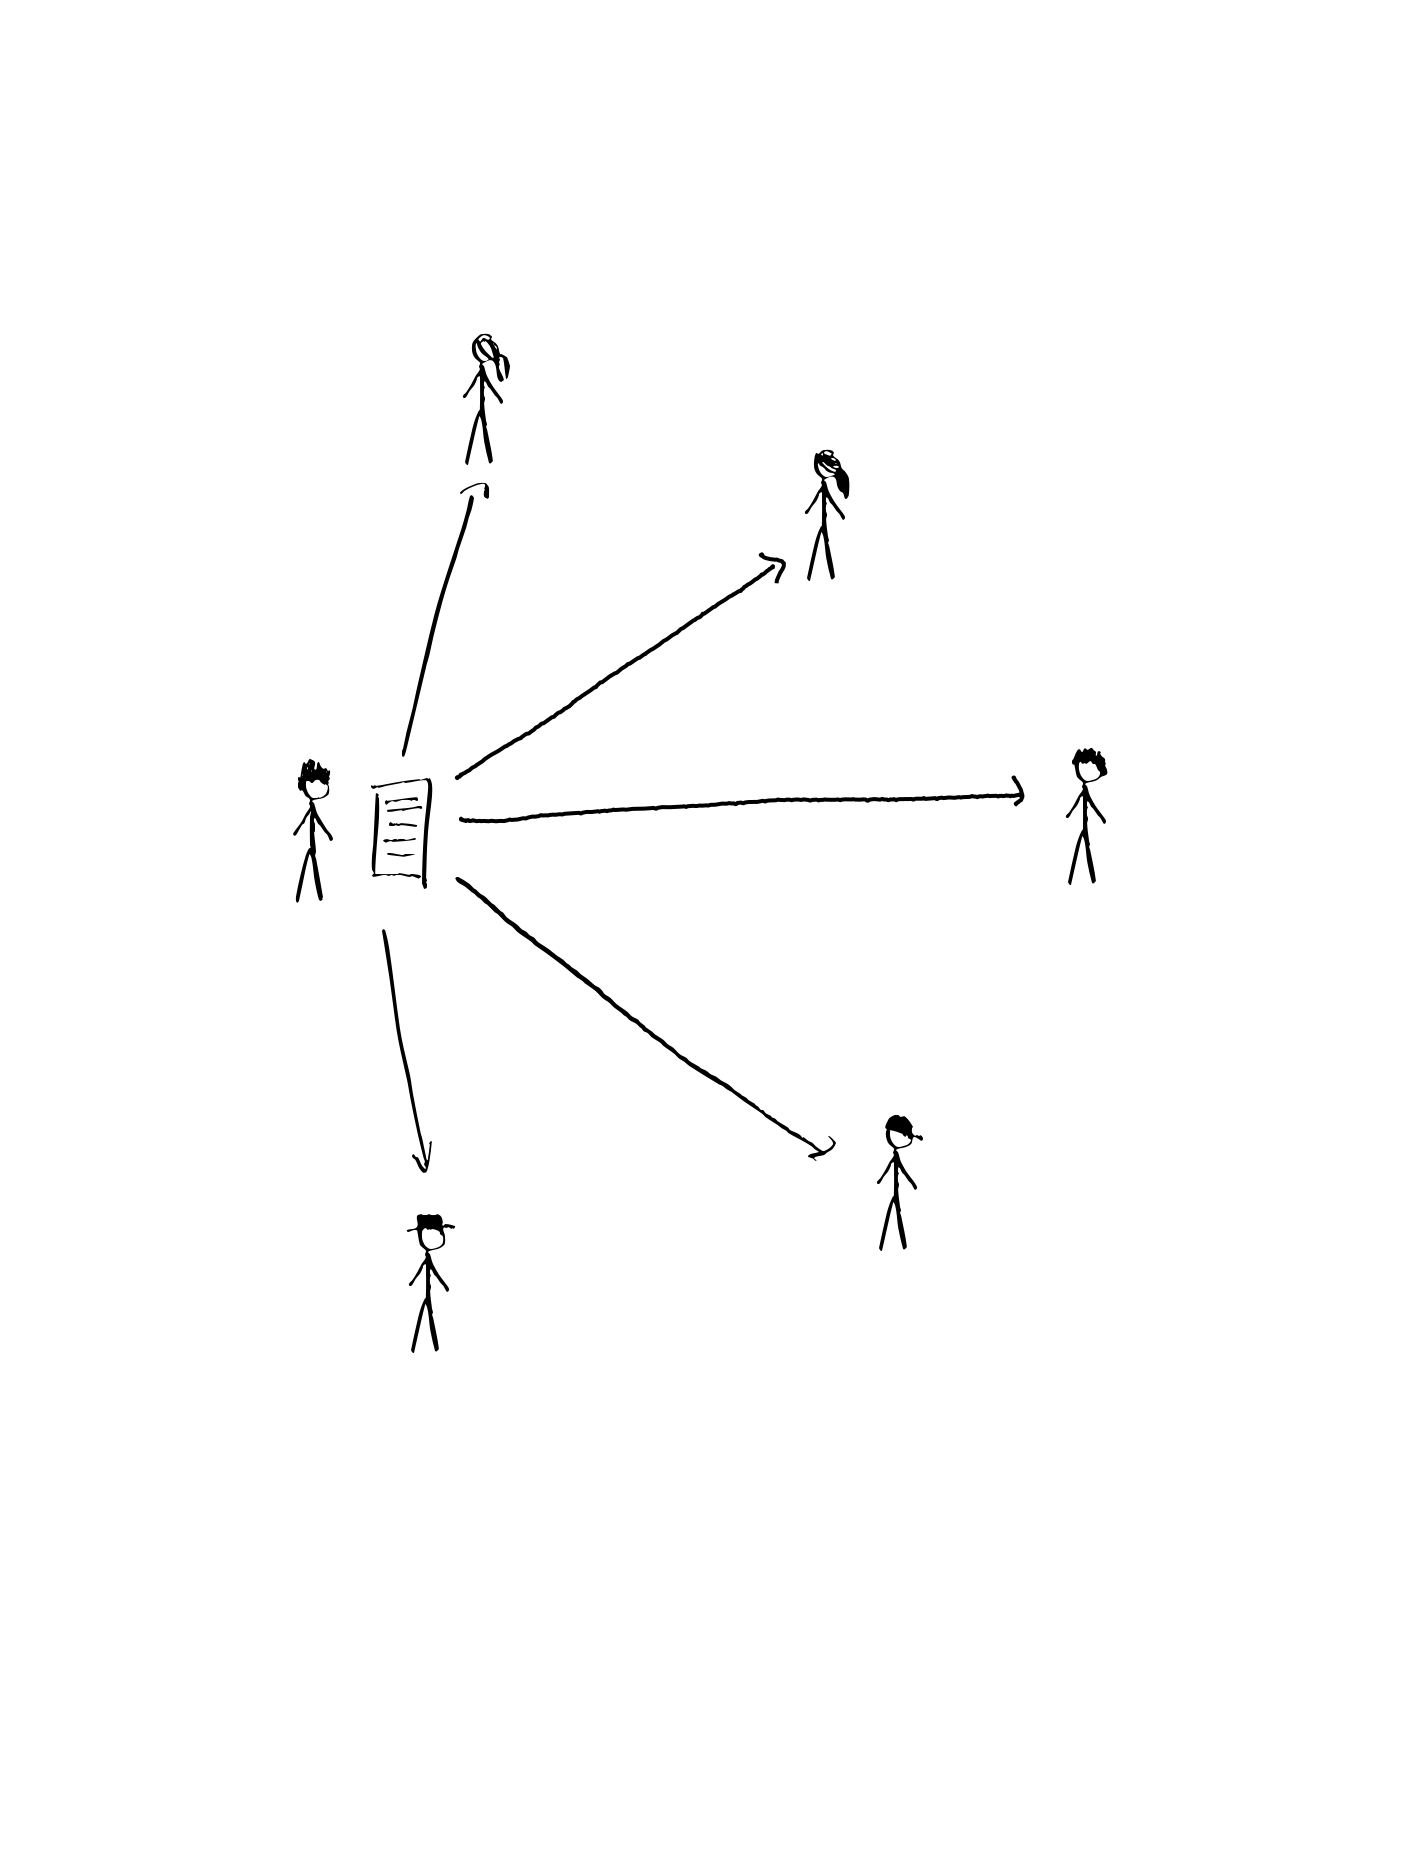
\includegraphics[height=0.4\textheight]{fig/centralized.pdf}
      \caption{Centralized}
    \end{subfigure}
    \hfill
    \begin{subfigure}{0.45\columnwidth}
      \centering
      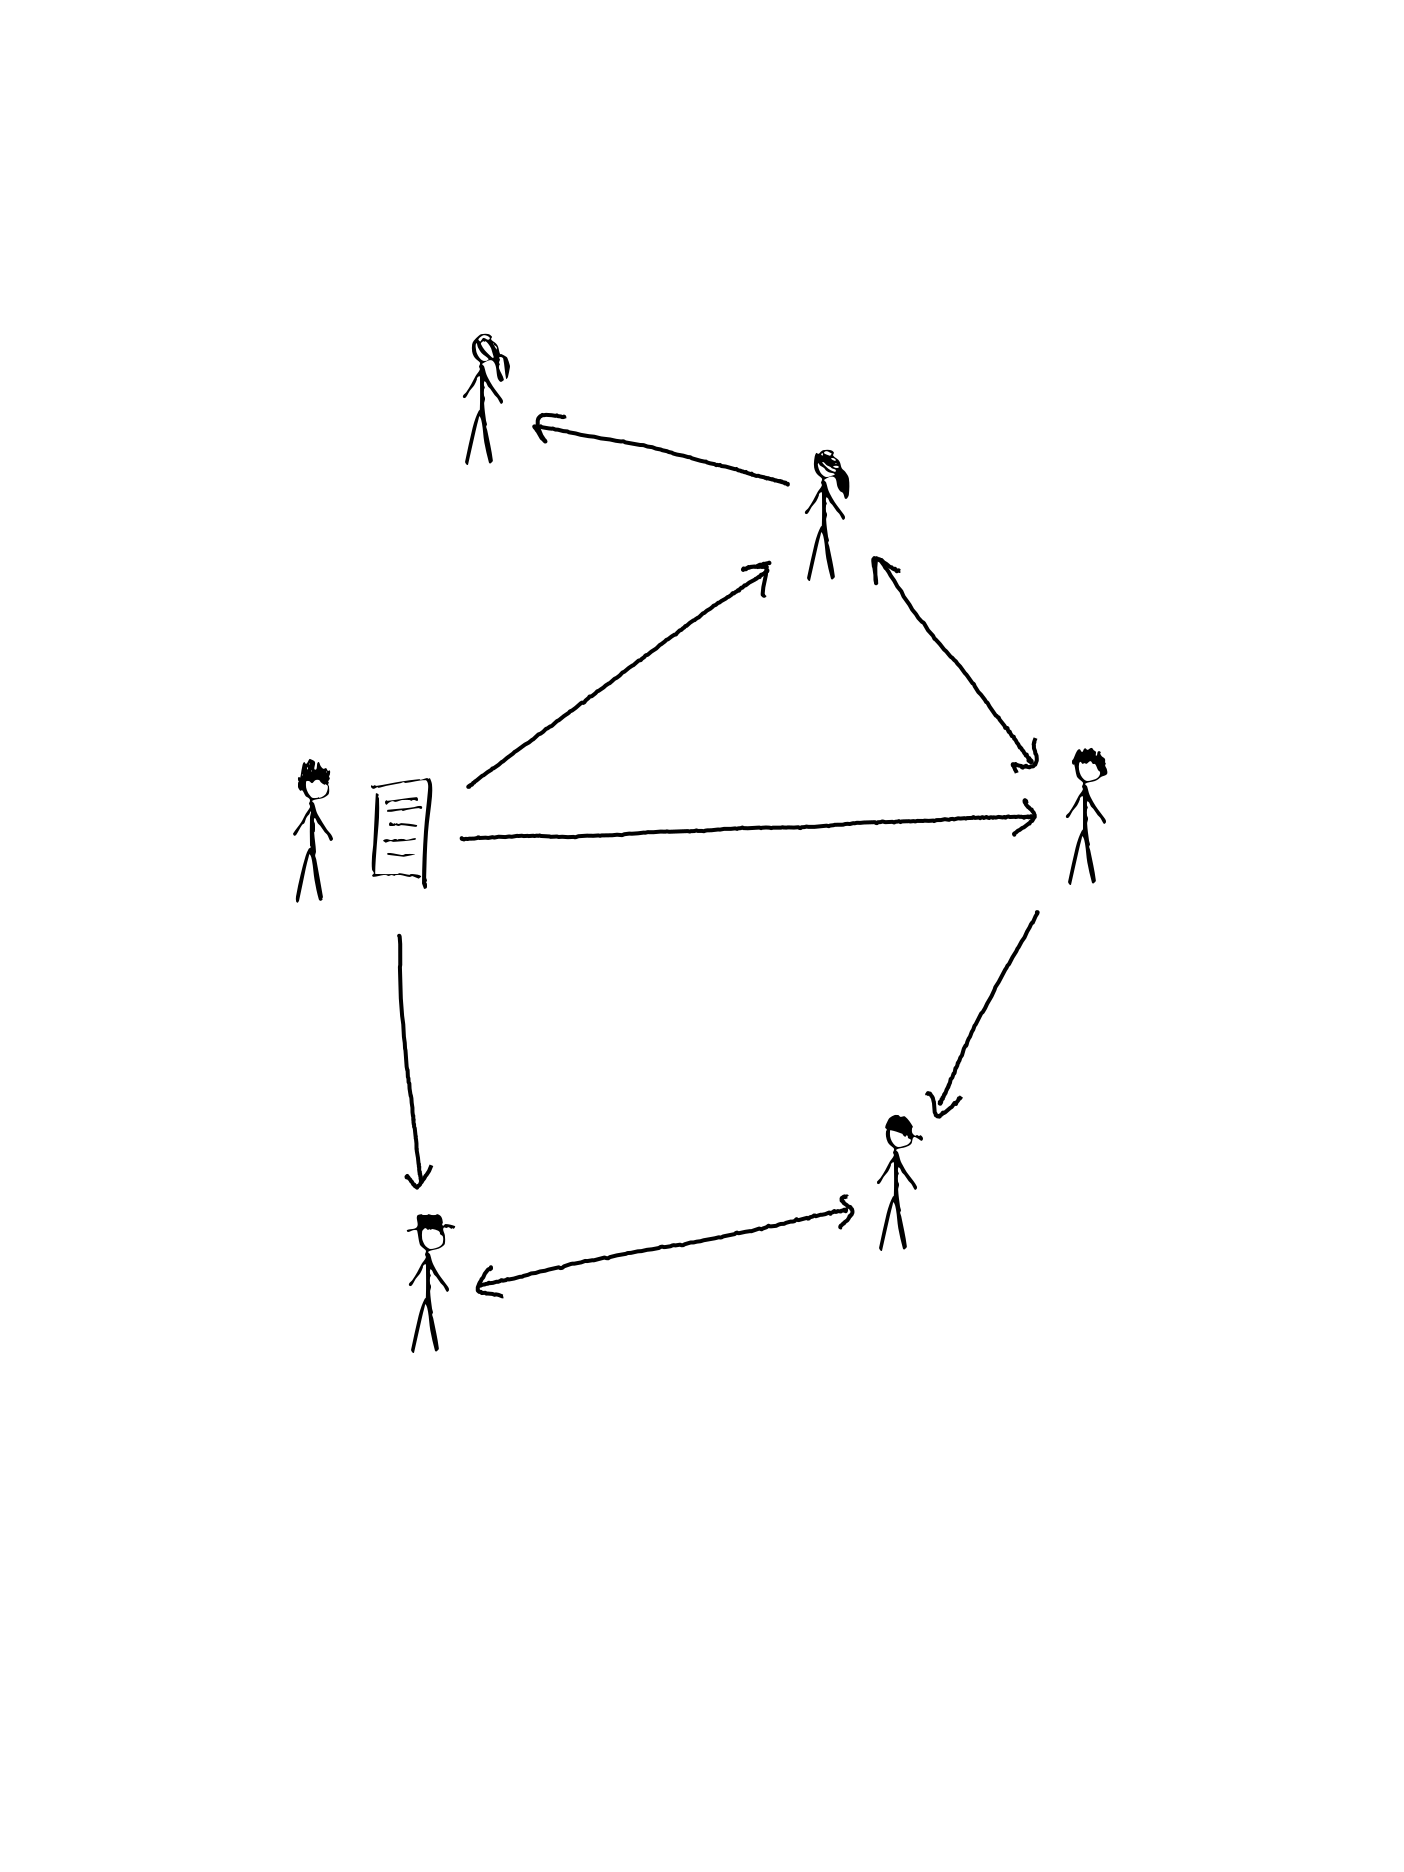
\includegraphics[height=0.4\textheight]{fig/p2p.pdf}
      \caption{Peer-to-peer (P2P)}
    \end{subfigure}
  \end{figure}

  \begin{question}
    \begin{itemize}
      \item How to get most out of the P2P case?
    \end{itemize}
  \end{question}
\end{frame}

\begin{frame}
  \begin{figure}
    \begin{subfigure}{0.45\columnwidth}
      \centering
      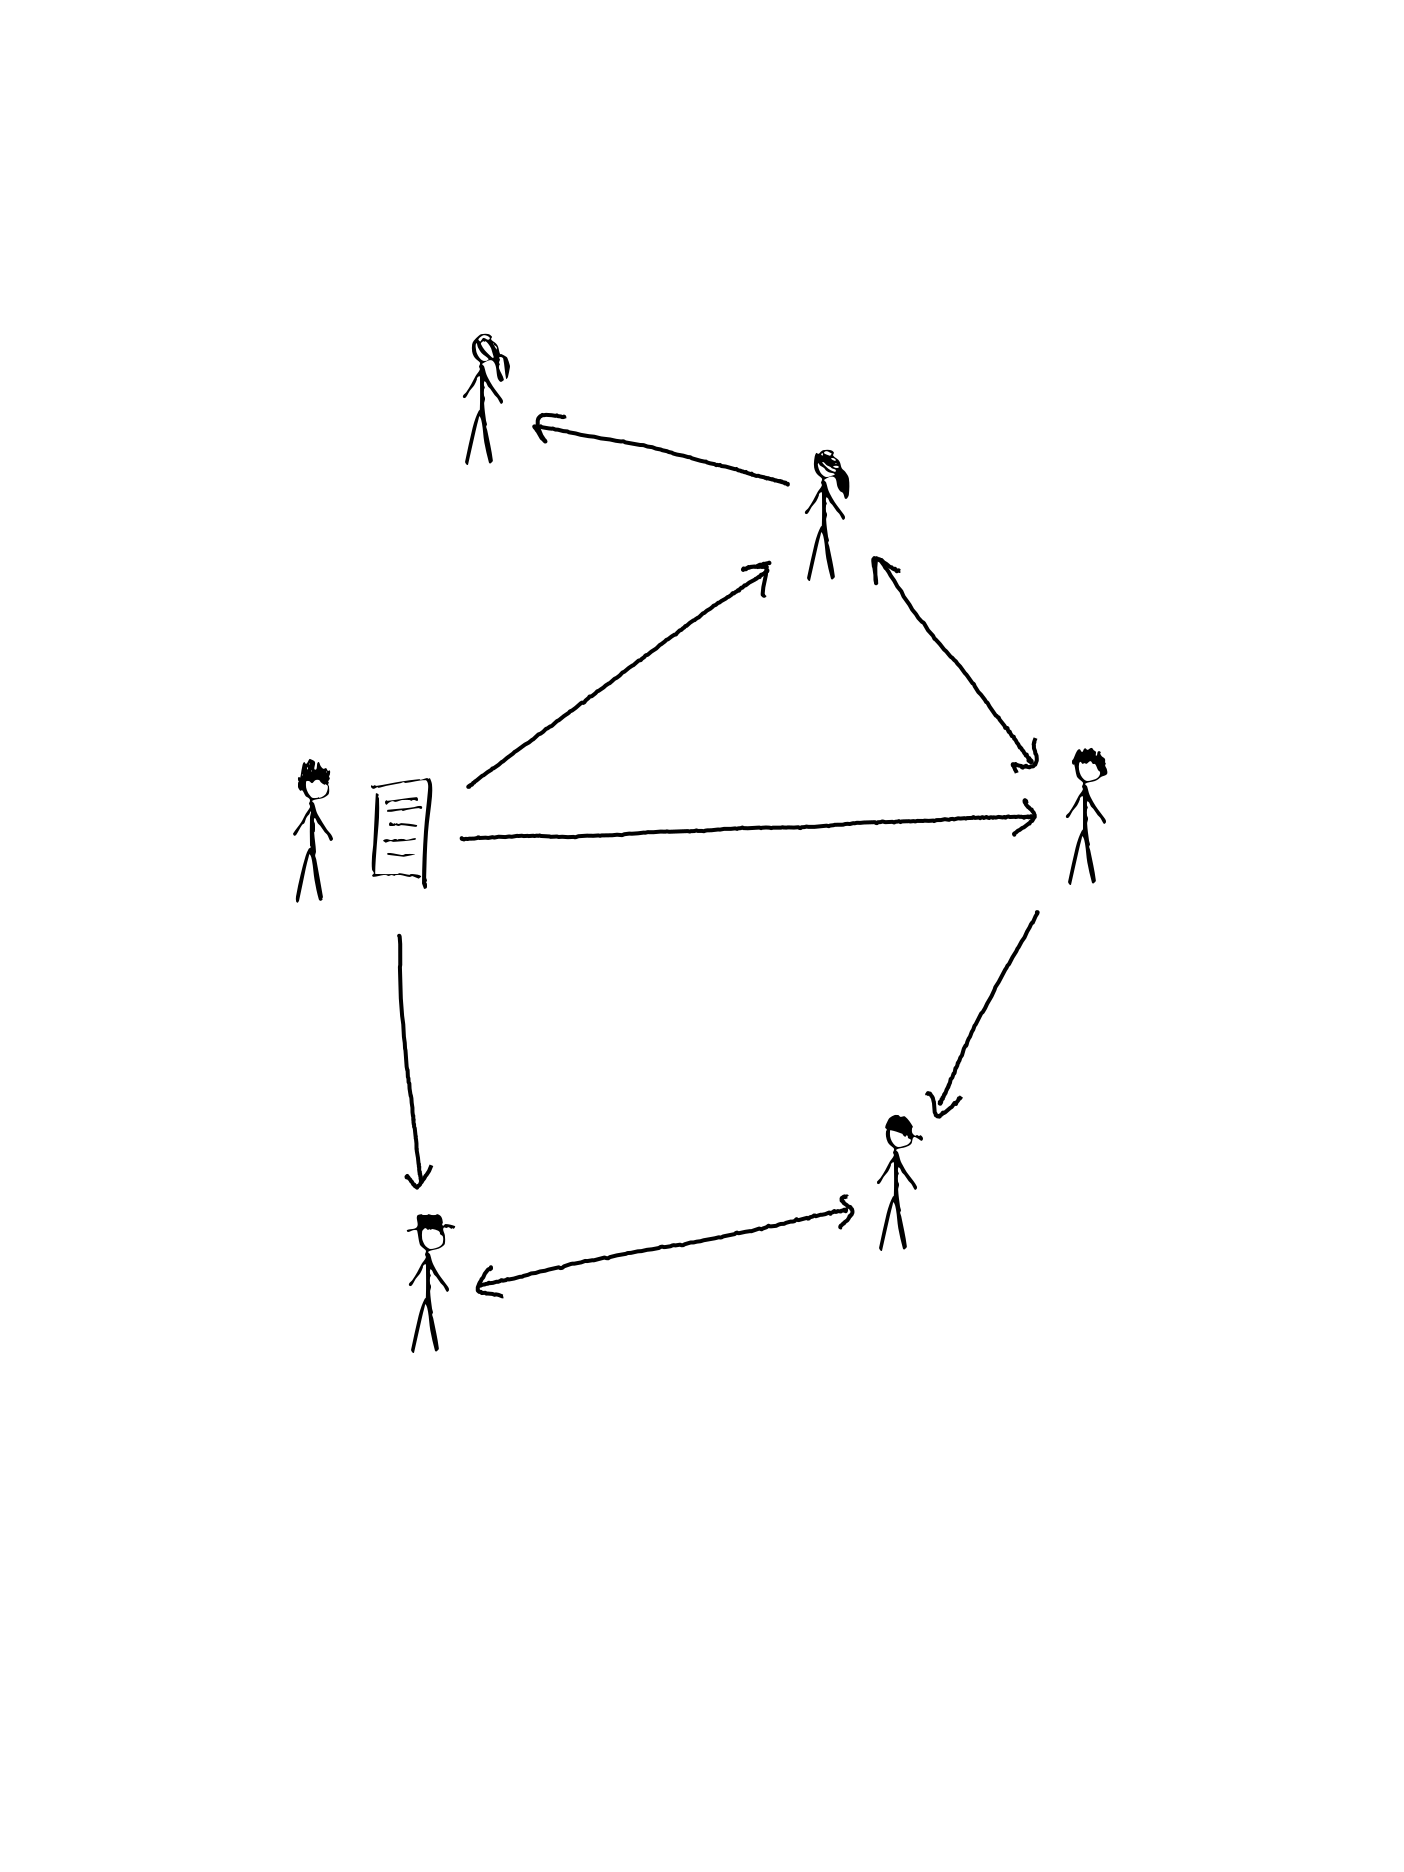
\includegraphics[height=0.5\textheight]{fig/p2p.pdf}
      \caption{Peer-to-peer (P2P)}
    \end{subfigure}
    \hfill
    \begin{subfigure}{0.45\columnwidth}
      \only<1>{%
        \centering
        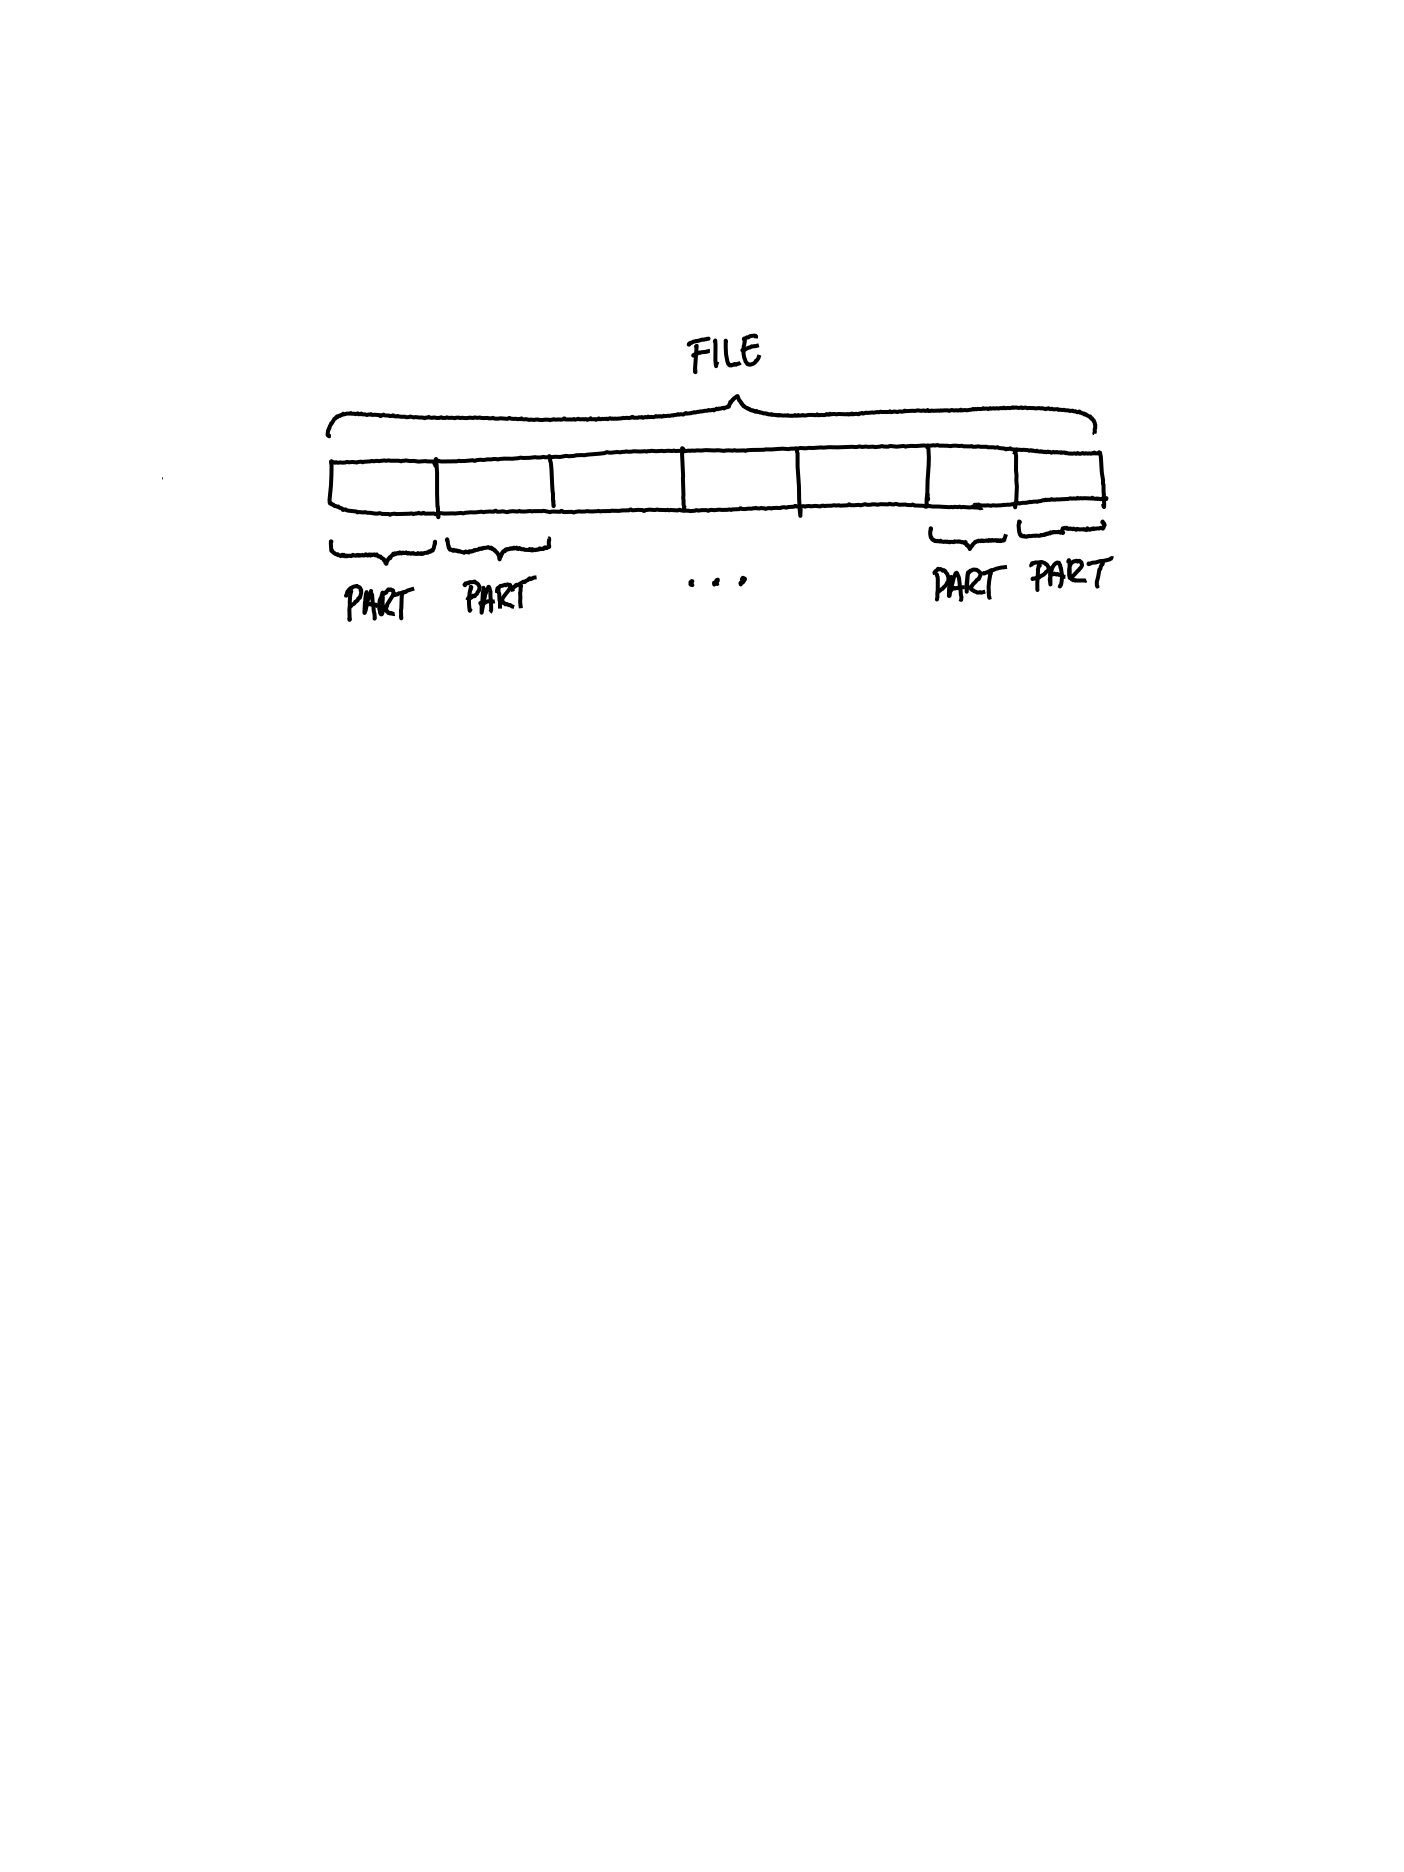
\includegraphics[width=\columnwidth]{fig/file-parts.pdf}
        \caption{File divided into parts}
      }
      \only<2>{%
        \centering
        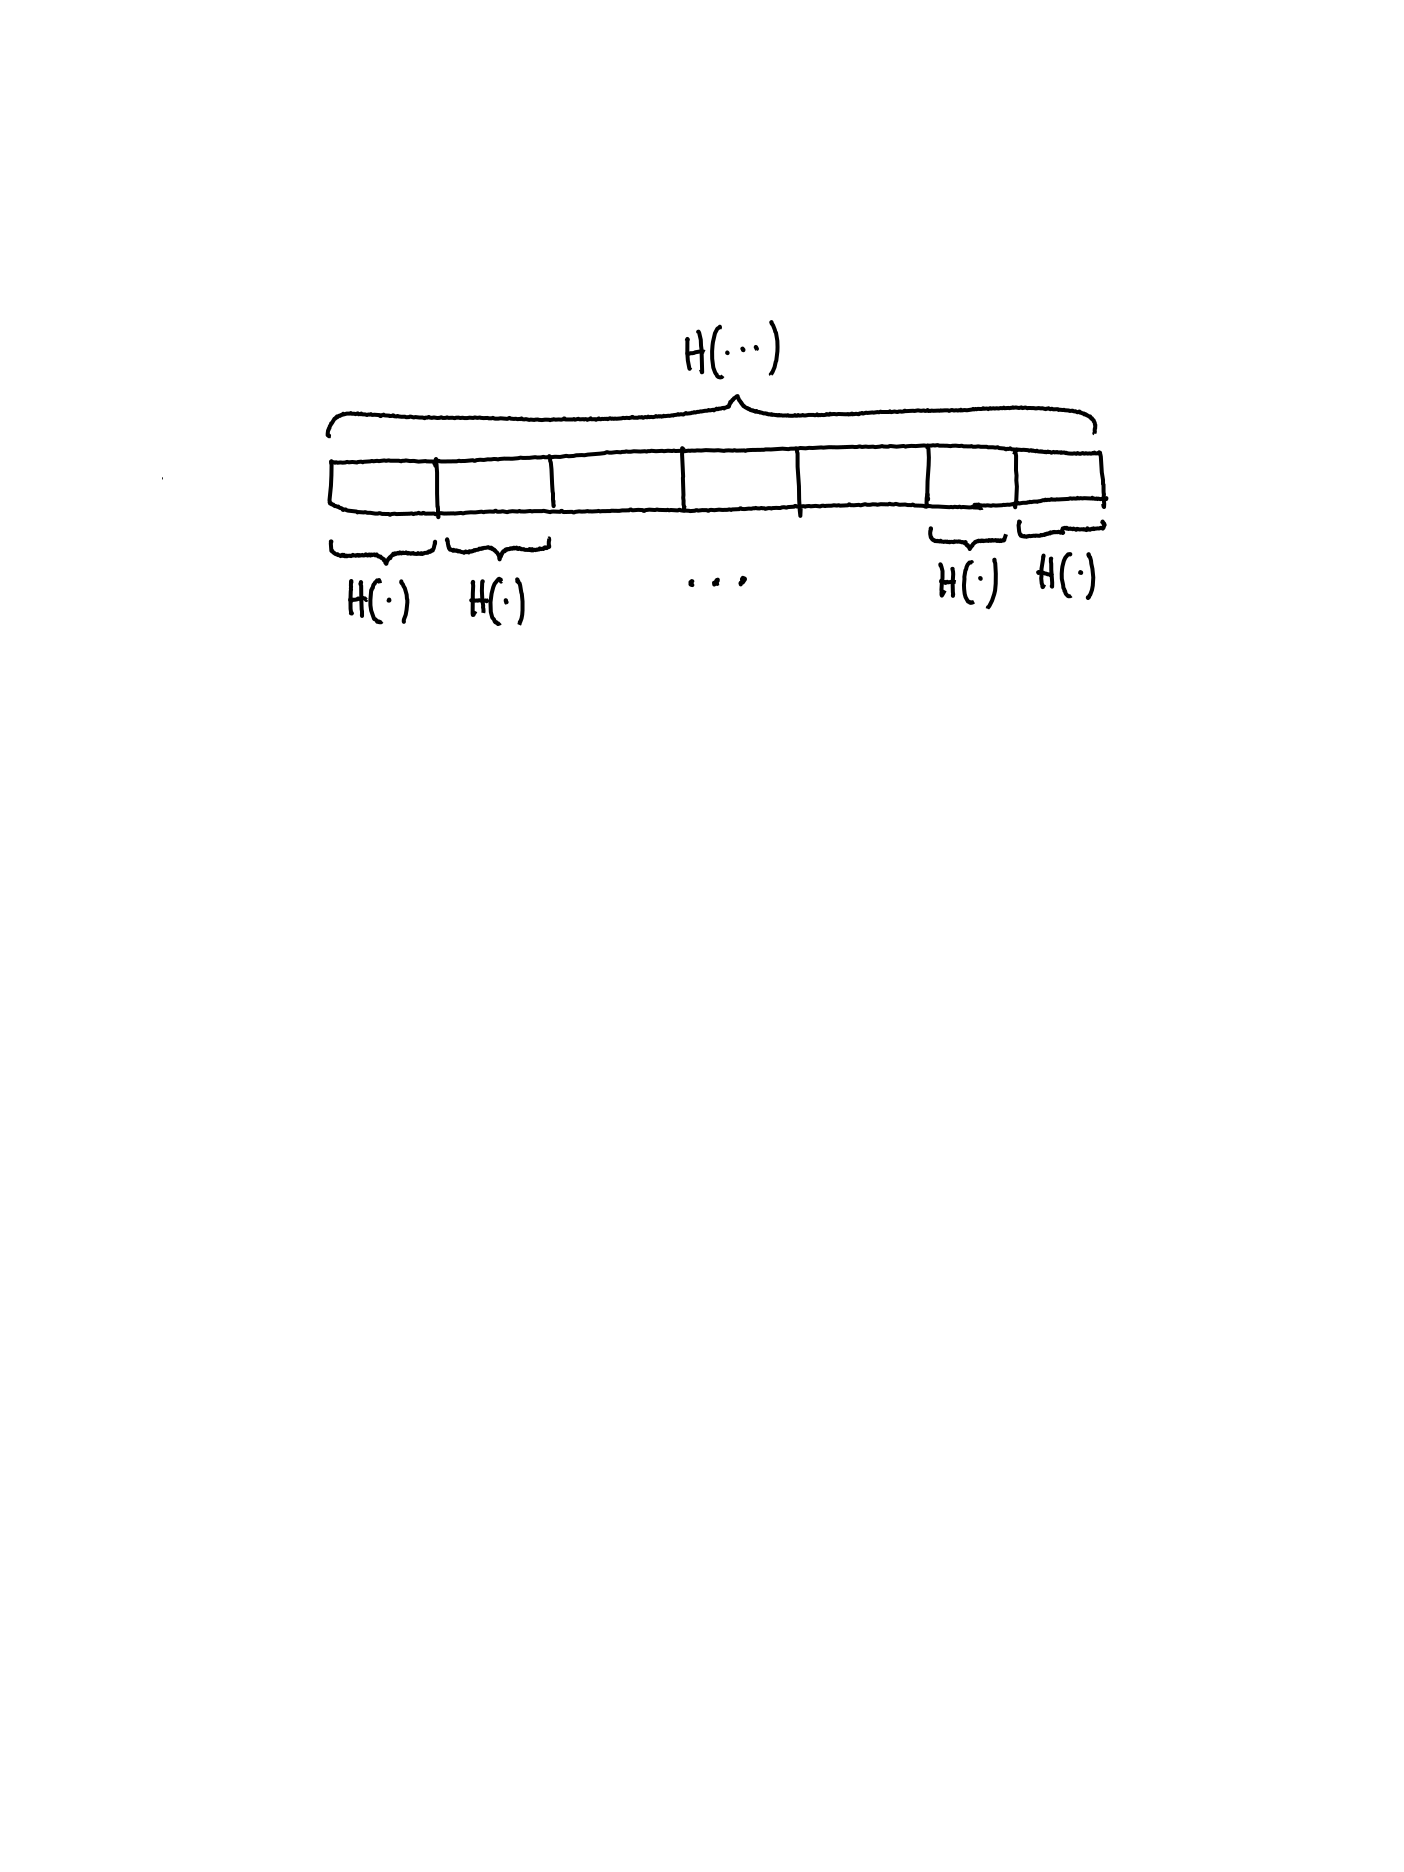
\includegraphics[width=\columnwidth]{fig/torrent-hashes.pdf}
        \caption{Hash values of file and parts}
      }
    \end{subfigure}
  \end{figure}

  \begin{solution}
    \begin{itemize}
      \item Must keep track of different parts of a file.
    \end{itemize}
  \end{solution}
\end{frame}

\begin{frame}
  \begin{remark}
    \begin{itemize}
      \item We want a cryptographic hash function if we want authenticity 
        properties.
      \item Will a malicious actor inject fake parts of files?
      \item Authenticated torrent file gives authenticated file.
    \end{itemize}
  \end{remark}
\end{frame}


\subsection{Git}

\begin{frame}
  \begin{remark}
    \begin{itemize}
      \item Git is a content-addressable file system.
    \end{itemize}
  \end{remark}

  \pause

  \begin{definition}[Git blob {[binary large object]}]
    \begin{itemize}
      \item Name is hash value of content and a header.
      \item Content is just the content.
    \end{itemize}
  \end{definition}
\end{frame}

\begin{frame}
  \begin{figure}
    \centering
    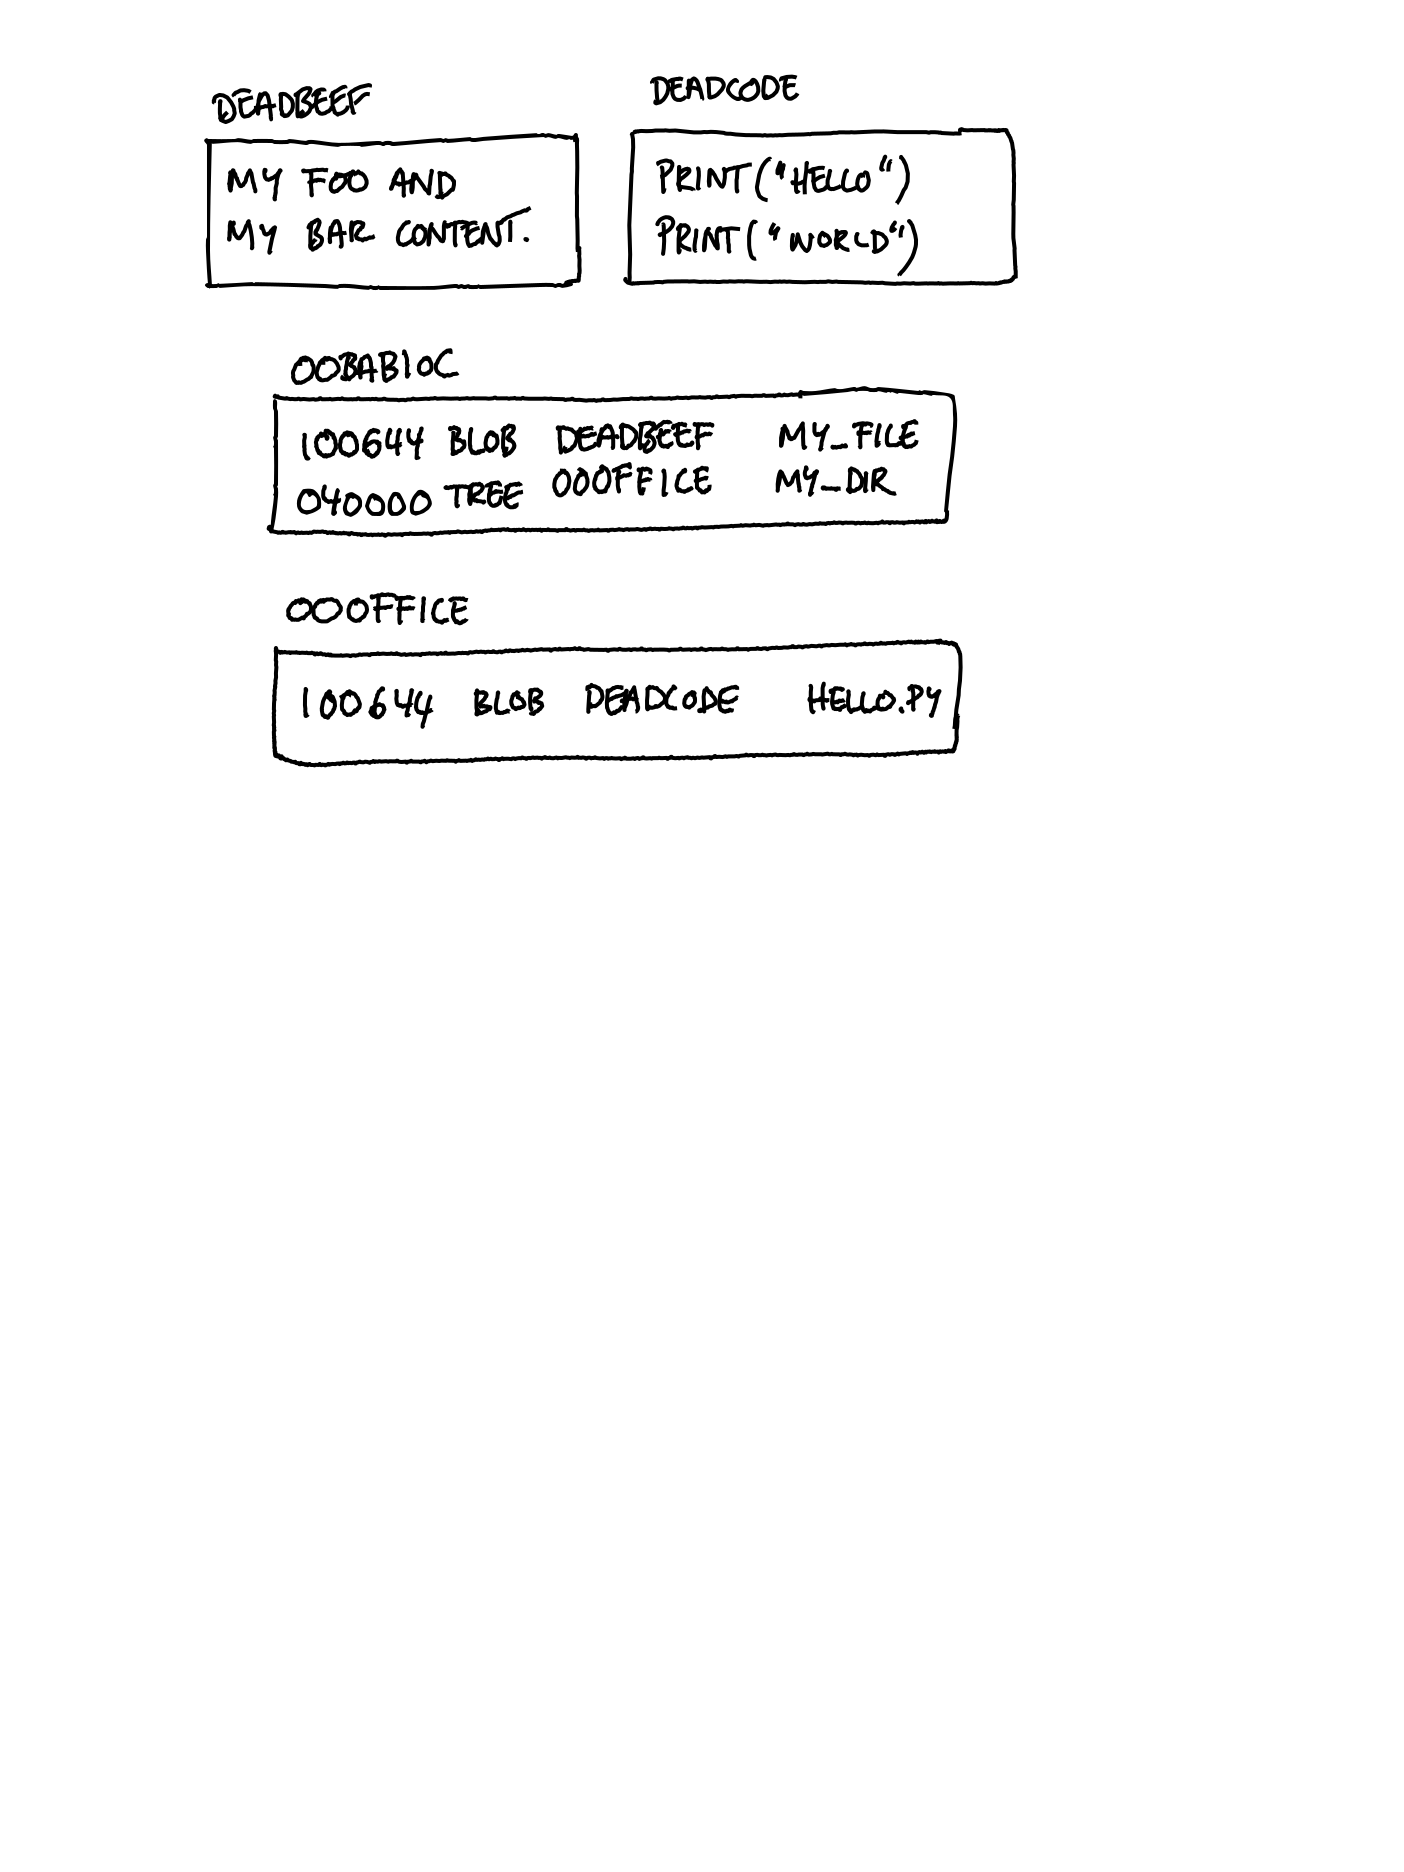
\includegraphics[height=0.8\textheight]{fig/git-objects.pdf}
    \caption{Git objects with hashes \texttt{deadbeef}, \texttt{deadcode}, 
    \texttt{oobab1oc}, \texttt{000ff1ce}.}
  \end{figure}
\end{frame}

\begin{frame}
  \begin{remark}
    \begin{itemize}
      \item Blobs don't store file names etc., just content.
      \item Tree objects solve the problem of storing the filename.
      \item Also allow you to store a group of files together.
    \end{itemize}
  \end{remark}

  \pause

  \begin{definition}[Tree object]
    \begin{itemize}
      \item Blob with structured content:
      \item file mode
      \item type (blob, tree \etc)
      \item human readable name
    \end{itemize}
  \end{definition}
\end{frame}

\begin{frame}
  \begin{figure}
    \centering
    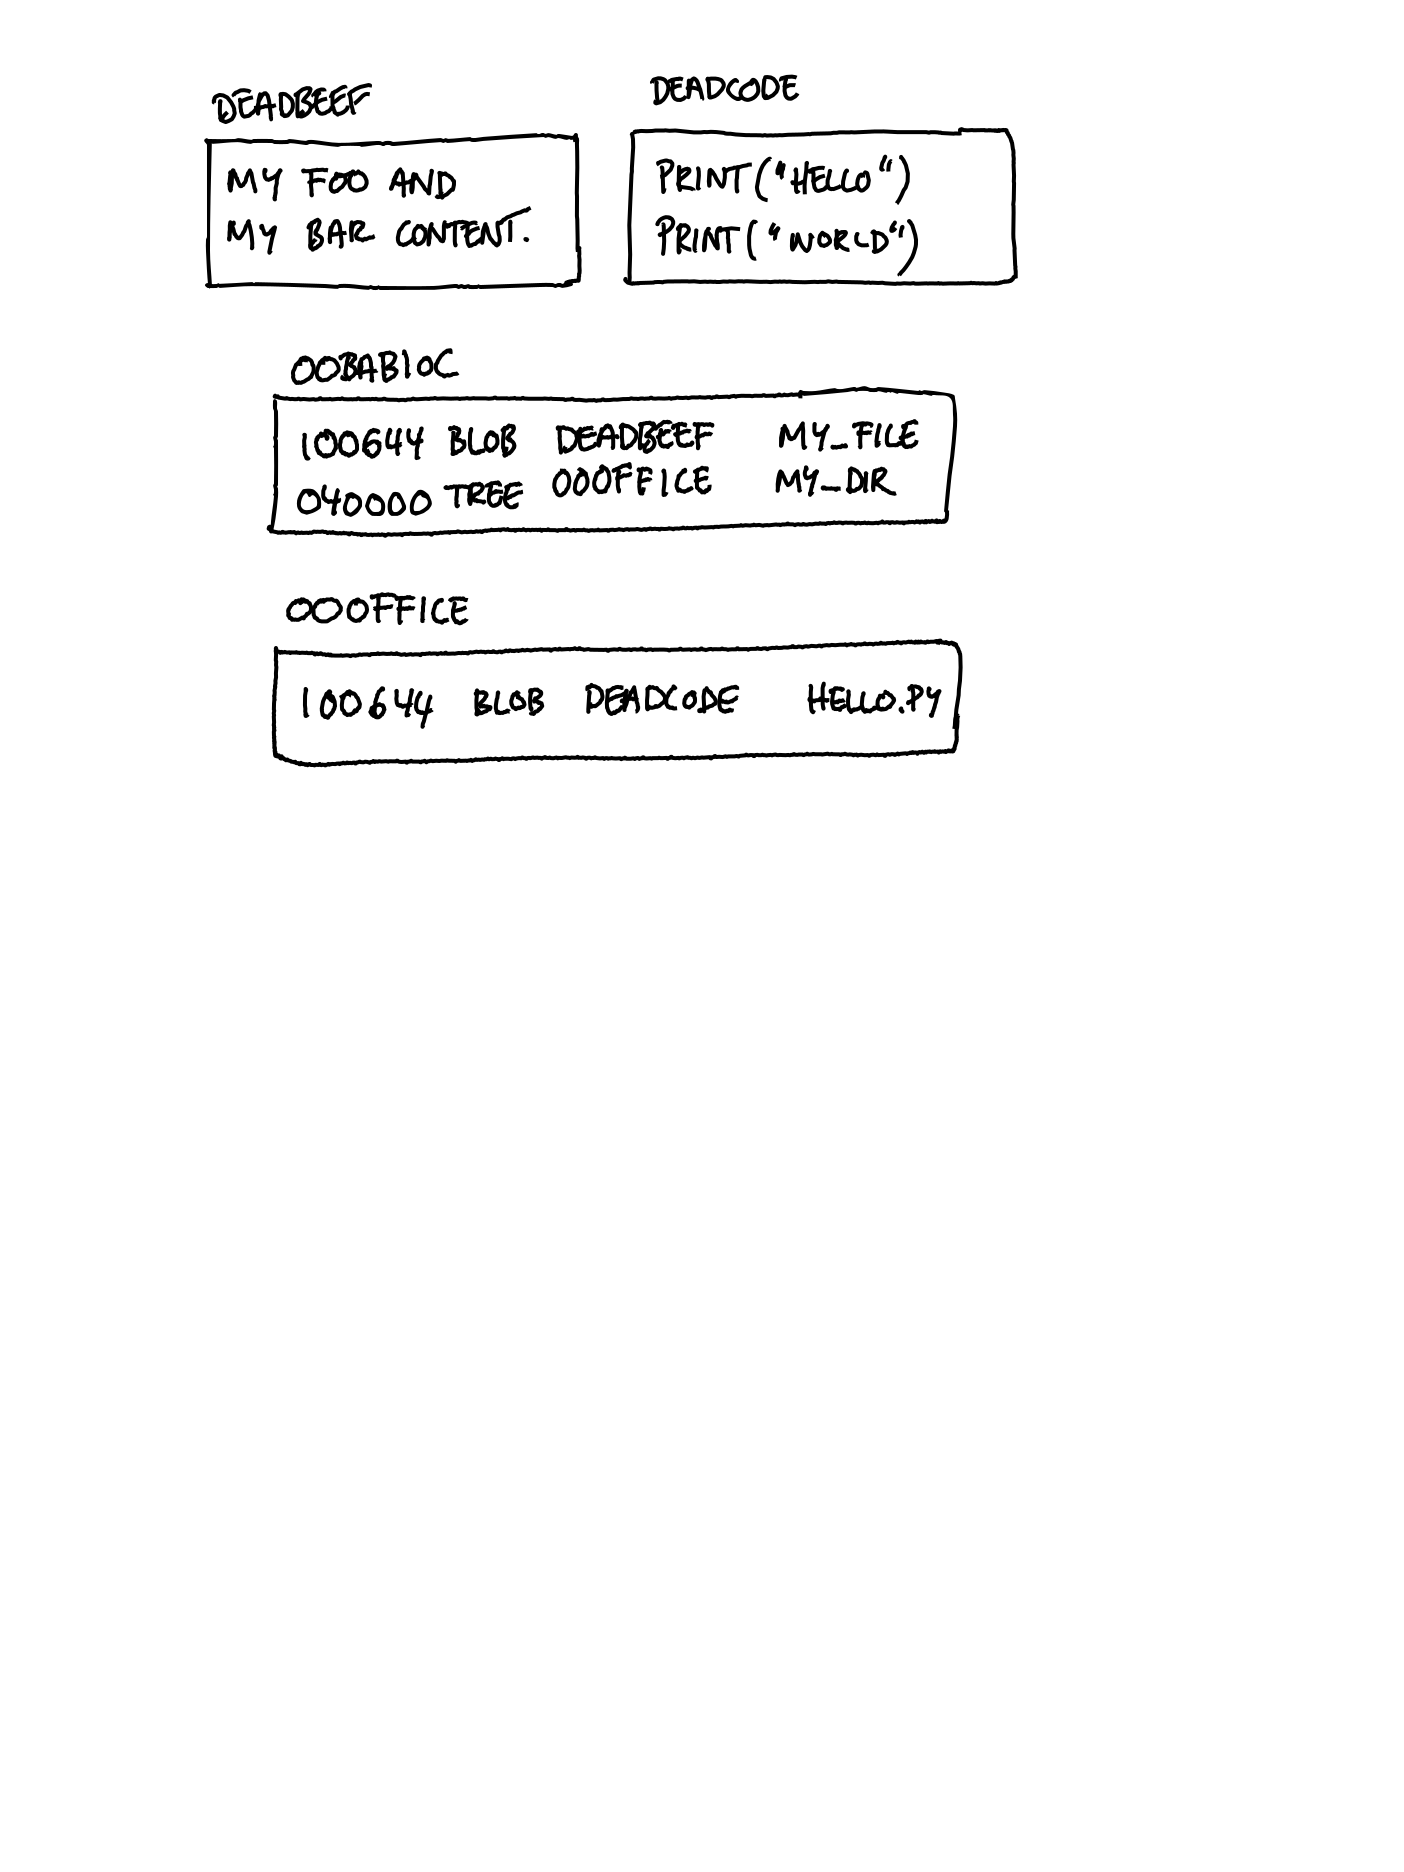
\includegraphics[height=0.8\textheight]{fig/git-objects.pdf}
    \caption{Tree objects with hashes \texttt{oobab1oc}, \texttt{000ff1ce}.}
  \end{figure}
\end{frame}

\begin{frame}
  \begin{remark}
    \begin{itemize}
      \item A tree doesn't keep track of versions.
    \end{itemize}
  \end{remark}

  \begin{definition}[Commit]
    \begin{itemize}
      \item Tree (current state)
      \item Parent commits
      \item Author
      \item Commit log
    \end{itemize}
  \end{definition}
\end{frame}

\begin{frame}
  \begin{figure}
    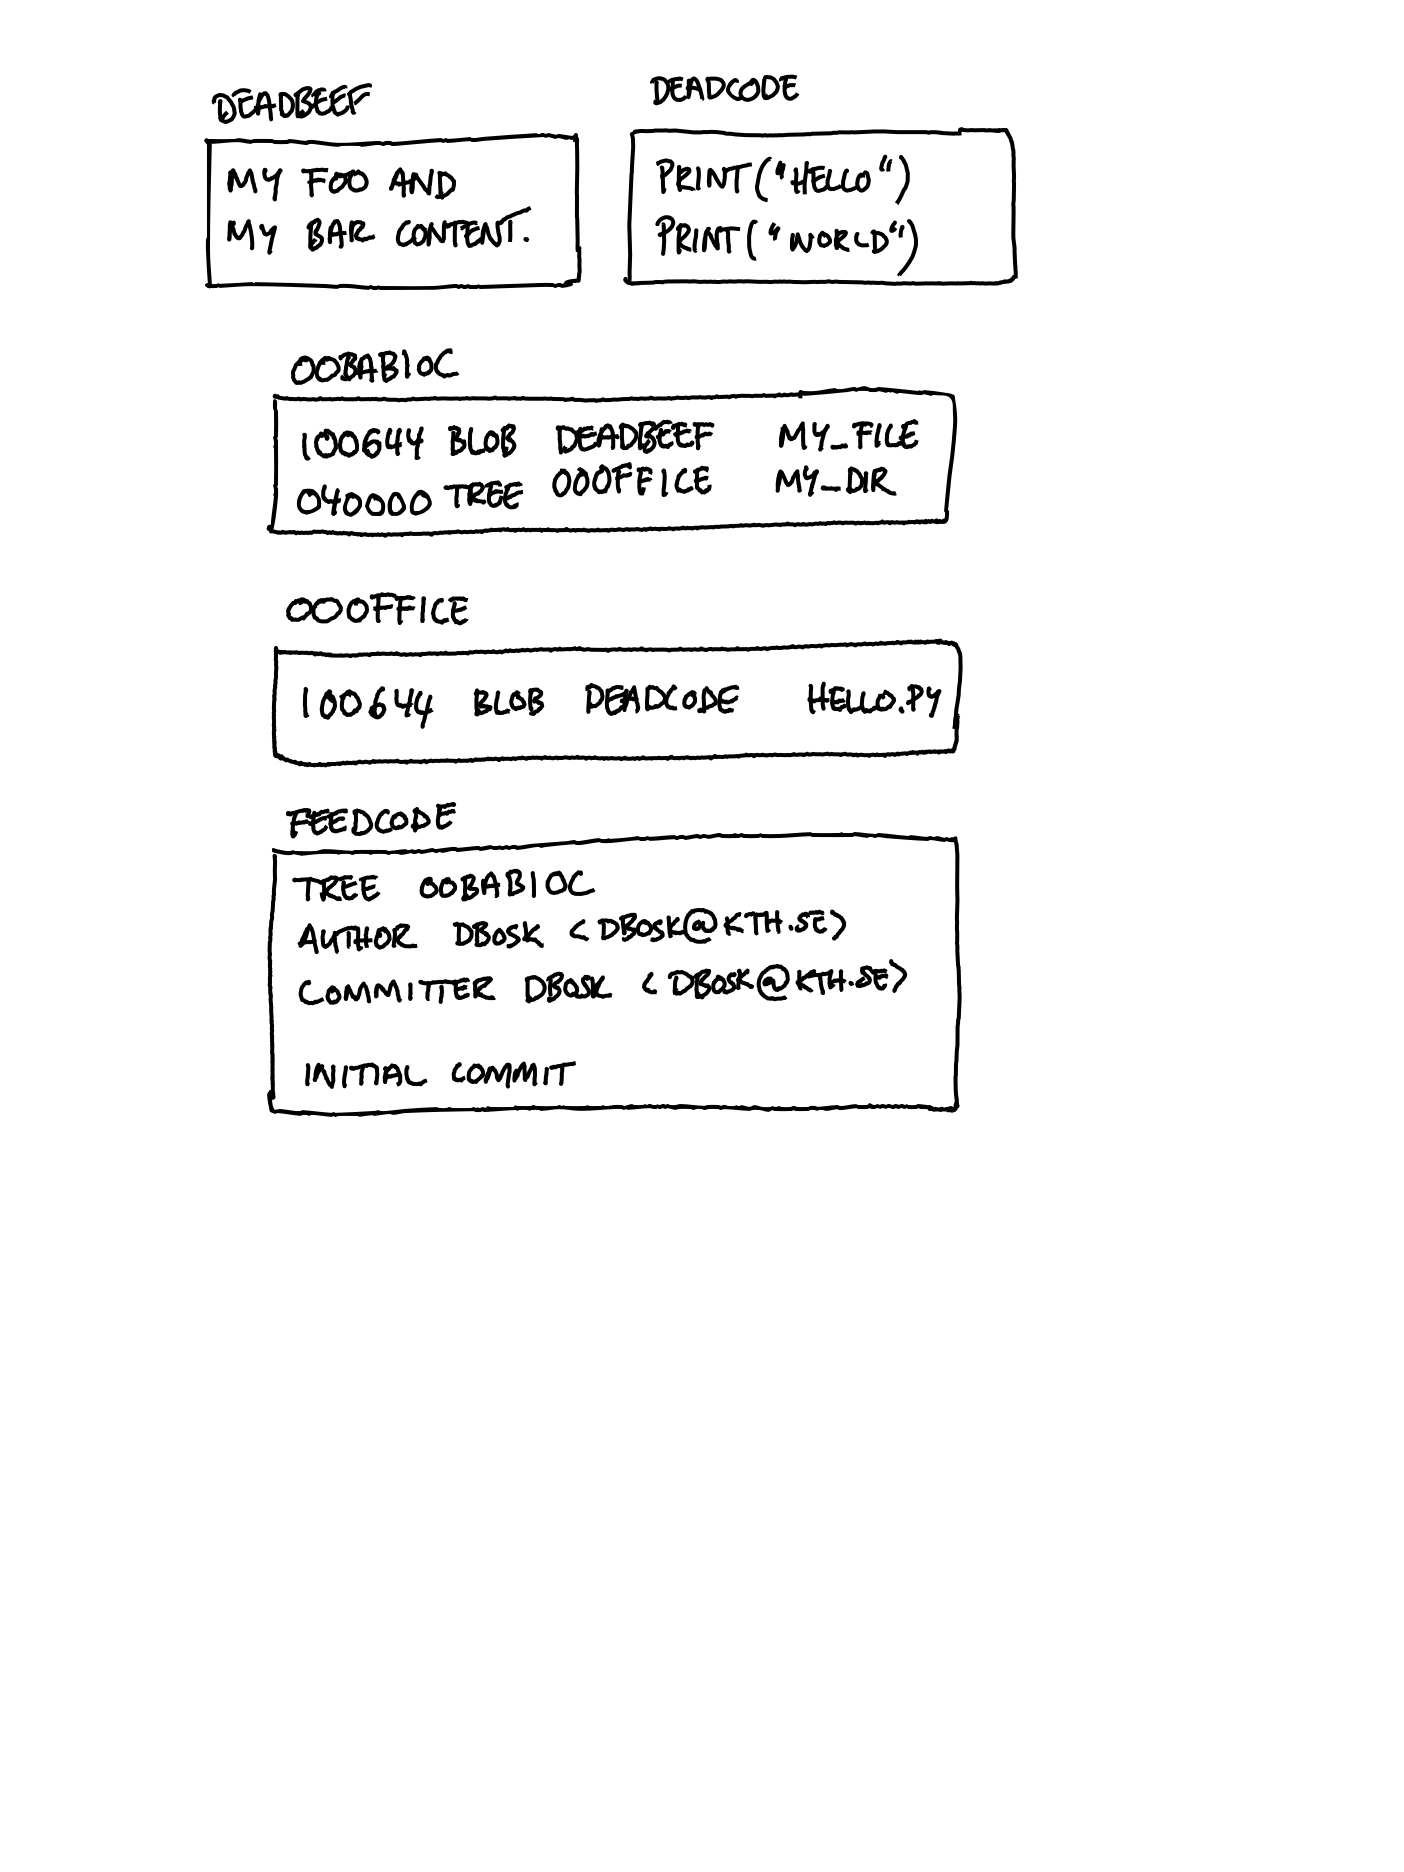
\includegraphics[height=0.8\textheight]{fig/git-commit.pdf}
    \caption{A commit \texttt{feedc0de}.}
  \end{figure}
\end{frame}

\begin{frame}
  \begin{exercise}
    \begin{columns}
      \begin{column}{0.40\columnwidth}
        \begin{figure}
          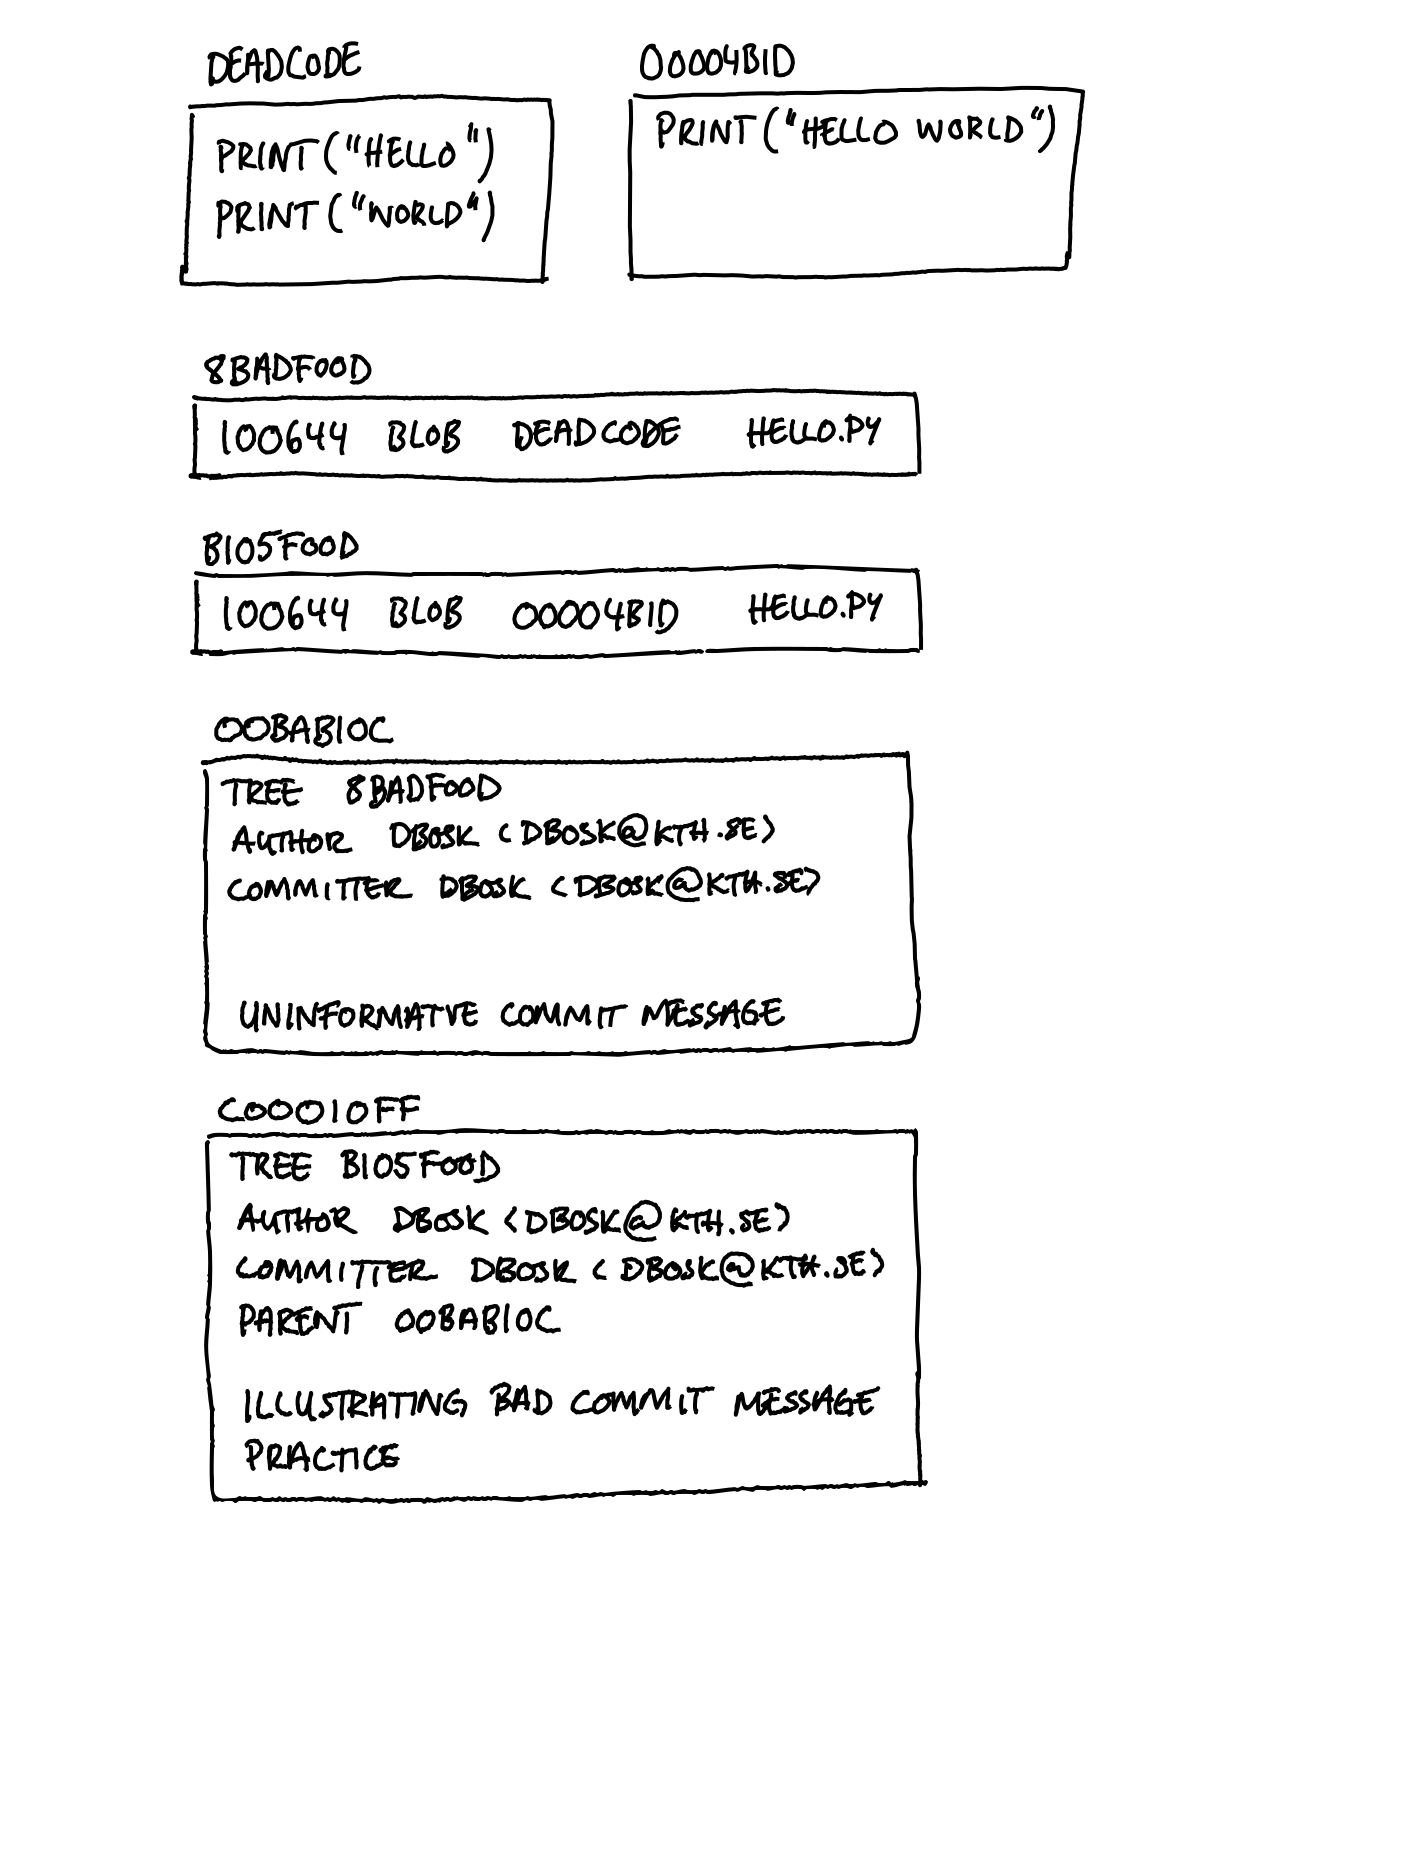
\includegraphics[height=0.6\textheight]{fig/git-challenge-2.pdf}
          \caption{Some Git objects.}
        \end{figure}
      \end{column}
      \begin{column}{0.45\columnwidth}
        \begin{itemize}
          \item What happened if the initial commit is \texttt{00bab10c}?
        \end{itemize}
      \end{column}
    \end{columns}
  \end{exercise}
\end{frame}

%\begin{frame}
%  \begin{exercise}
%    \begin{columns}
%      \begin{column}{0.40\columnwidth}
%        \begin{figure}
%          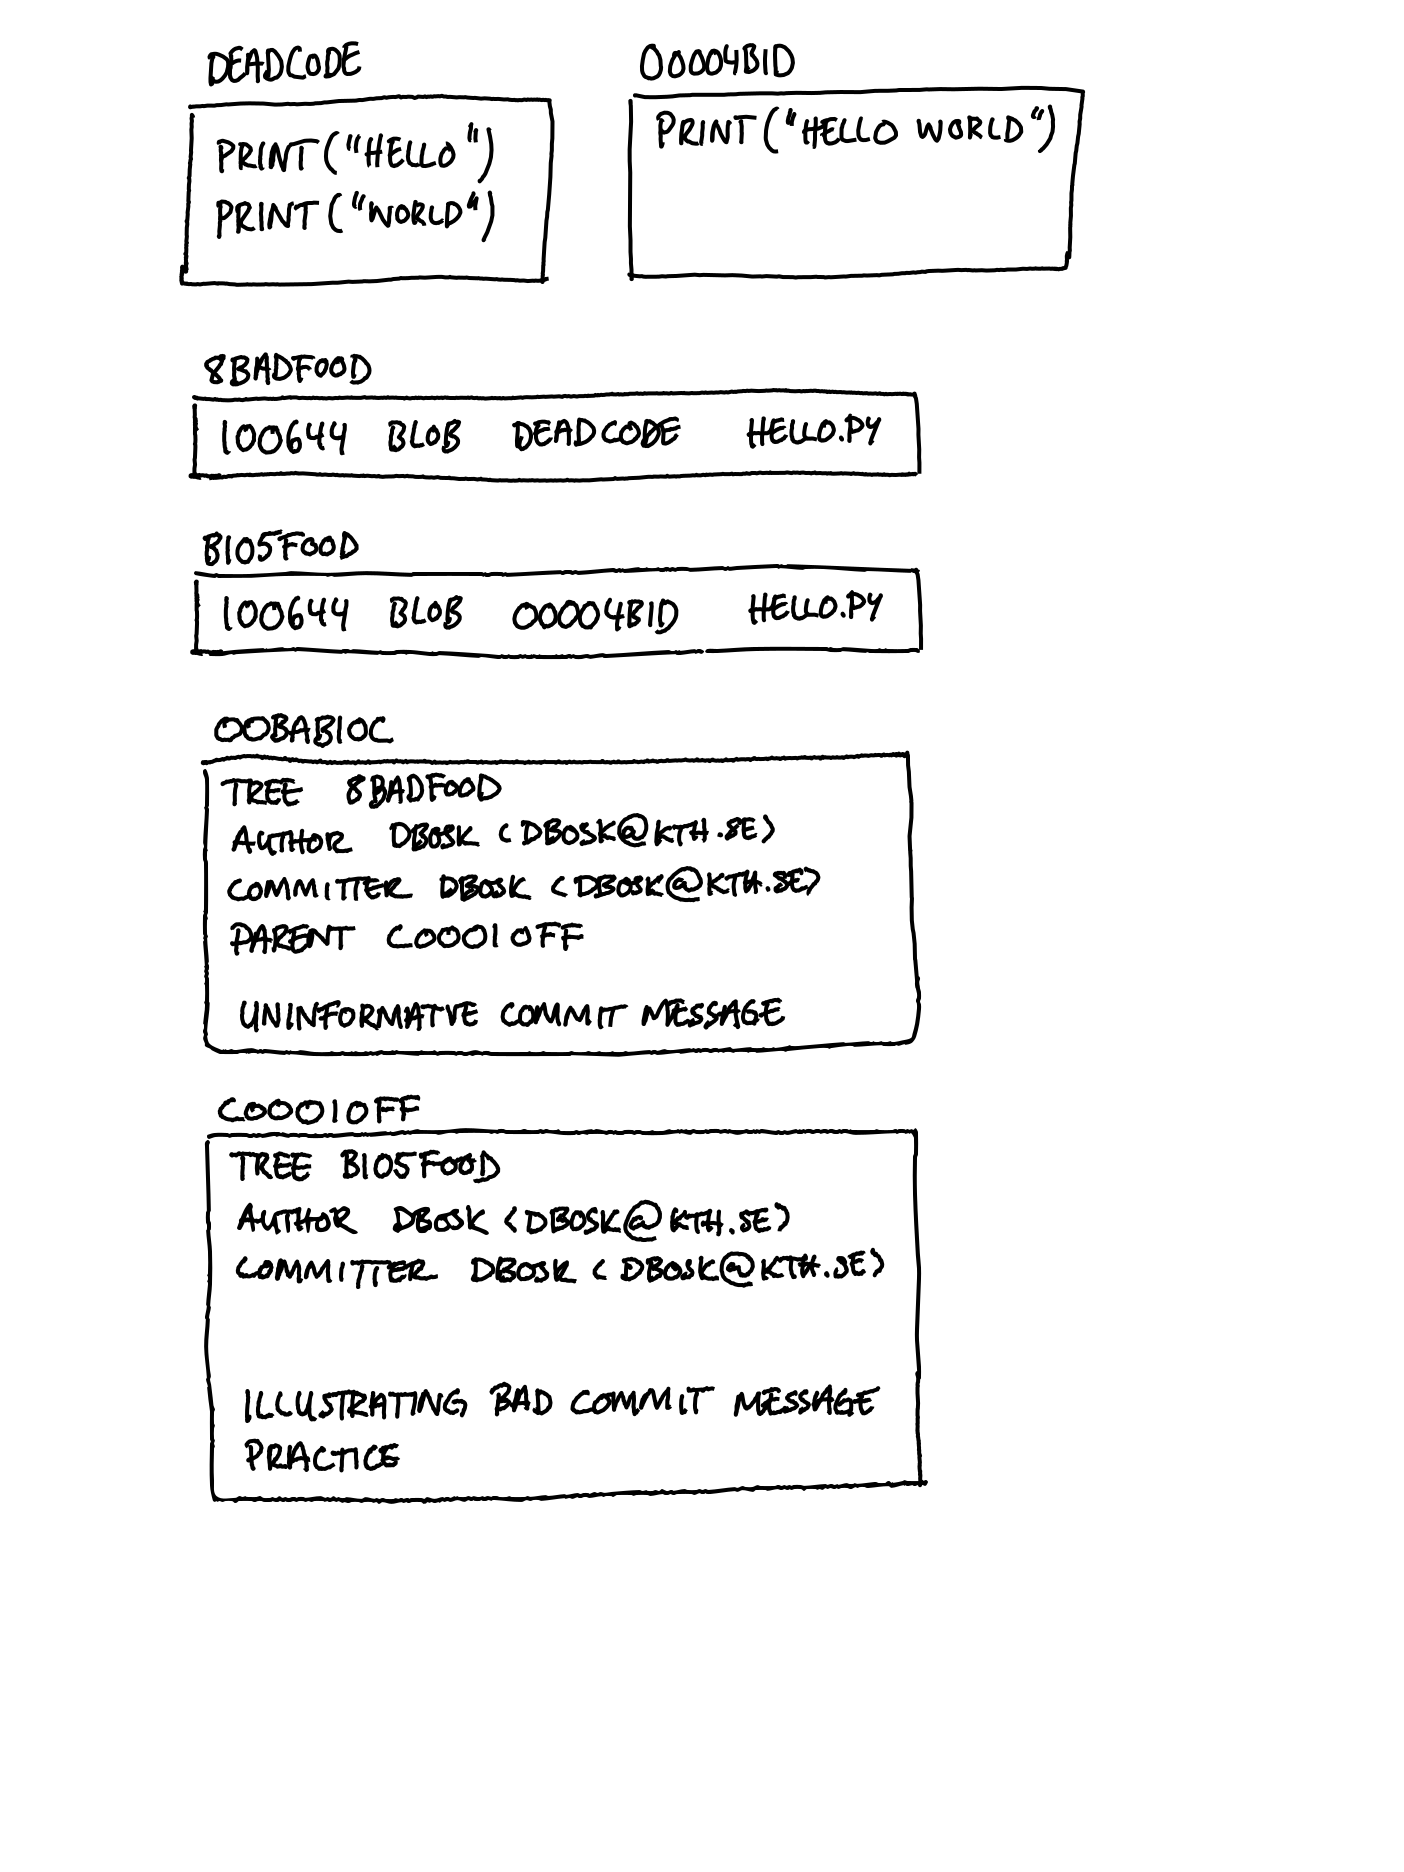
\includegraphics[height=0.6\textheight]{fig/git-challenge-1.pdf}
%          \caption{Some Git objects.}
%        \end{figure}
%      \end{column}
%      \begin{column}{0.45\columnwidth}
%        \begin{itemize}
%          \item What happened if the initial commit is \texttt{c00010ff}?
%        \end{itemize}
%      \end{column}
%    \end{columns}
%  \end{exercise}
%\end{frame}

\begin{frame}
  \begin{exercise}
    \begin{itemize}
      \item What properties do we want from the hash function?
    \end{itemize}
  \end{exercise}
\end{frame}

\begin{frame}
  \begin{solution}
    \begin{itemize}
      \item Compression (short identifiers)
      \item Collision resistance:
        \begin{itemize}
          \item Cryptographic: in case we want authentication.
          \item Otherwise, just to avoid two different objects colliding.
        \end{itemize}
    \end{itemize}
  \end{solution}
\end{frame}
